\section{Econometrics Final 2019 / 20}

{
\subsection*{Watson}

{
\subsubsection*{Exercise 1}

\begin{enumerate}[label=(\alph*)]
{\item 
$$
\begin{aligned}
\varepsilon_{t} & =\frac{1-\phi L}{1-\theta L} y_{t} \\
& =(1-\phi L)\left(1+\theta L+(\theta L)^{2}+(\theta L)^{3}+\ldots\right) y_{t} \\
& =\left(1-\phi L+\theta L-\phi \theta L^{2}+(\theta L)^{2}-\phi \theta^{2} L^{3}+(\theta L)^{3}-\phi \theta^{3} L^{4}+\ldots\right) y_{t} \\
& =\left(1+(\theta-\phi) L+\theta(\theta-\phi) L^{2}+\theta^{2}(\theta-\phi) L^{3}+\ldots\right) y_{t} \\
& =y_{t}+(\theta-\phi)\left[y_{t-1}+\theta y_{t-2}+\theta^{2} y_{t-3}+\ldots\right]
\end{aligned}
$$

Thus, if we know $\phi$ and $\theta$ and all $y_{t-i} \forall i \geqslant 0$, were able to reconstruct $\varepsilon_{t}$.
}
{\item 
$$
\begin{aligned}
& \varepsilon_{t} \sim N(0,1) \\
& y_{t}\left|\varepsilon_{t}=\phi_{y_{t}-1}+\varepsilon_{t}\right| \varepsilon_{t} \sim N\left(\varepsilon_{t}, \frac{\phi^{2}}{1-\phi^{2}}\right) \\
& \Rightarrow\left(\begin{array}{l}
y_{t} \\
\varepsilon_{t}
\end{array}\right) \sim N\left(\left[\begin{array}{l}
0 \\
0
\end{array}\right],\left[\begin{array}{cc}
\frac{1}{1-\phi^{2}} & 1 \\
1 & 1
\end{array}\right]\right) \\
& \mathbb{E}\left(\varepsilon_{t} \mid y_{t}=2\right)=0+2\left(1-\phi^{2}\right)=2(1-0.64)=0.72
\end{aligned}
$$
}
\end{enumerate}
}
{
\subsubsection*{Exercise 2}

\begin{enumerate}[label=(\alph*)]
{\item 
$$
\begin{aligned}
g_{t} & =\left(\rho x_{t-1}+e_{t}\right)\left(\phi u_{t-1}+\varepsilon_{t}\right) \\
& =\rho \phi\left(x_{t-1} u_{t-1}\right)+\phi u_{t-1} e_{t}+\rho x_{t-1} \varepsilon_{t}+e_{t} \varepsilon_{t} \\
& =\gamma g_{t-1}+a_{t}
\end{aligned}
$$

where $\gamma=\rho \phi ; a_{t}=\phi u_{t-1} e_{t}+\rho x_{t-1} \varepsilon_{t}+e_{t} \varepsilon_{t}$

Now, also $a_{t-1}=\phi u_{t-2} e_{t-1}+\rho x_{t-2} \varepsilon_{t-1}+e_{t-1} \varepsilon_{t-1}$

Note, that $\mathbb{E}\left(a_{t} a_{t-1}\right)=0$, as either $e_{t}$ or $\varepsilon_{t}$ will enter every part of the sum, and both are independent of the rest. This also holds for $\mathbb{E}\left(a_{t} a_{t-j}\right)$, where $j \geqslant 1$. Therefore, $a_t$ is serially uncorrelated.
}
{\item 
\begin{itemize}
    \item $\left\{y_{t}, x_{t}\right\}$ is ergodic \& stationary by $|\rho|<1$ \& $|\phi|<1$ 
    \item $\mathbb{E}\left(g_{t}\right)=0$ since $\mathbb{E}\left(x_{t}\right)=\mathbb{E}\left(u_{t}\right)=0$
    \item $\{g_t\}$ is not mds
\end{itemize}

\begin{enumerate}[label=(\arabic*)]
\item Construct estimator
$$
\begin{aligned}
\hat{\beta}_{OLS} & =\left(\frac{1}{T} \sum x_{t}^{2}\right)^{-1}\left(\frac{1}{T} \sum x_{t} y_{t}\right)=\left(\frac{1}{T} \sum x_{t}^{2}\right)^{-1}\left(\frac{1}{T} \sum \beta x_{t}^{2}+g_{t}\right) \\
& =\beta+\left(\frac{1}{T} \sum x_{t}^{2}\right)^{-1}\left(\frac{1}{T} \sum g_{t}\right)
\end{aligned}
$$
\item Show convergences

$$
\begin{aligned}
\left(\frac{1}{T} \sum x_{t}^{2}\right)^{-1} & \xrightarrow{p} \mathbb{E}\left(x_{t}^{2}\right)^{-1}=1-\rho^{2} \quad \text{by LLN \& CMT}\\
\frac{1}{\sqrt{T}} \sum {g_t} & \xrightarrow{d} N(0, \Omega) \quad \text{by CLT}
\end{aligned}
$$

\item Combine (1) \$ (2):

$$
\sqrt{T}(\hat{\beta}-\beta) \xrightarrow{d} N\left(0, \mathbb{E}\left(x_{t}^{2}\right)^{-1} \Omega \mathbb{E}\left(x_{t}^{2}\right)^{-1}\right)
$$
\item Find $\Omega$ :

First, the $MA (\infty)$ representation of $g_{t}$ is

$$
g_{t}=(1-\gamma L)^{-1} a_{t}
$$

Therefore, the ACGF gives us

$$
\Omega=\sum_{j=-\infty}^{\infty} \lambda_{j}=\left(\frac{1}{1-\gamma}\right)^{2} \operatorname{Var}\left(a_{t}\right)
$$

Now, we find $\operatorname{Var}\left(a_{t}\right)$:

$$
\begin{aligned}
\operatorname{Var}\left(a_{t}\right) & =\mathbb{E}\left[\left(\phi u_{t-1} e_{t}+\rho x_{t-1} \varepsilon_{t}+e_{t} \varepsilon_{t}\right)^{2}\right] \\
& =\mathbb{E}\left[\phi^{2} u_{t-1}^{2} e_{t}^{2}+\rho^{2} x_{t-1}^{2} \varepsilon_{t}^{2}+e_{t}^{2} \varepsilon_{t}^{2}\right] \text { by } e_{t} \perp \varepsilon_{t} \\
& =\phi^{2} \mathbb{E}\left[u_{t-1}^{2}\right]+\rho^{2} \mathbb{E}\left[x_{t-1}^{2}\right]+1 \\
& =\frac{\phi^{2}}{1-\phi^{2}}+\frac{\rho^{2}}{1-\rho^{2}}+1
\end{aligned}
$$
\item Express $V$:

$$
\begin{aligned}
V & =\Omega \mathbb{E}\left(x_{t}^{2}\right)^{-2}=\left(\frac{1}{1-\gamma}\right)^{2}\left[\frac{\phi^{2}}{1-\phi^{2}}+\frac{\rho^{2}}{1-\rho^{2}}+1\right]\left(1-\rho^{2}\right)^{2} \\
& =\frac{\phi^{2}\left(1-\rho^{2}\right)+\rho^{2}\left(1-\phi^{2}\right)+\left(1-\rho^{2}\right)\left(1-\phi^{2}\right)}{\left(1-\phi^{2}\right)\left(1-\rho^{2}\right)(1-\gamma)^{2}}\left(1-\rho^{2}\right)^{2} \\
& =\frac{1-\rho^{2} \phi^{2}}{\left(1-\phi^{2}\right)(1-\gamma)^{2}}\left(1-\rho^{2}\right)=\frac{(1-\gamma)(1+\gamma)}{\left(1-\phi^{2}\right)(1-\gamma)^{2}}\left(1-\rho^{2}\right) \\
& =\frac{1+\gamma}{1-\gamma} \frac{1-\rho^{2}}{1-\phi^{2}}
\end{aligned}
$$
\end{enumerate}
}
\end{enumerate}
}
{
\subsubsection*{Exercise 3}

\begin{enumerate}[label=(\alph*)]
{\item 
$$
\begin{aligned}
& \min _{b} \sum_{t=1}^{T}\left(y_{t}-x_{t} b\right)^{2}+\lambda b^{2} \\
& \min _{b} \sum_{t=1}^{T} y_{t}^{2}-b \cdot 2 \sum_{t=1}^{T} y_{t} x_{t}+b^{2} \sum_{t=1}^{T} x_{t}^{2}+b^{2} \lambda
\end{aligned}
$$

$$
F O C: \quad-2 \sum_{t=1}^{\top} y_{t} x_{t}+2 b \sum_{t=1}^{T} x_{t}^{2}+2 b \lambda=0
$$

$$
\Leftrightarrow b=\left(\lambda+\sum_{t=1}^{T} x_{t}^{2}\right)^{-1}\left(\sum_{t=1}^{T} y_{t} x_{t}\right) \equiv \tilde{\beta}
$$
}
{\item 
$$
\begin{aligned}
\mathbb{E}\left(\tilde{\beta} \mid \left\{ x_{t}\right\}_{t=1}^{T}\right) & =\mathbb{E}\left(\left(\lambda+\sum_{t=1}^{T} x_{t}^{2}\right)^{-1}\left(\sum_{t=1}^{T} x_{t}\left(x_{t} \beta+\varepsilon_{t}\right)\right) \mid \left\{ x_{t}\right\}_{t=1}^{T}\right) \\
& =\mathbb{E}\left(\left(\lambda+\sum_{t=1}^{T} x_{t}^{2}\right)^{-1}\left(\sum_{t=1}^{T} x_{t}^{2} \beta+x_{t} \varepsilon_{t}\right) \mid \left\{ x_{t}\right\}_{t=1}^{T}\right) \\
& =\left(\lambda+\sum_{t=1}^{T} x_{t}^{2}\right)^{-1}\left(\sum_{t=1}^{T} x_{t}^{2} \beta\right) \neq \beta \quad \text{if } \lambda \neq 0
\end{aligned}
$$

Yes, the estimator is biased. $\lambda$ "punishes" large values (in absolute terms) of $\tilde{\beta}$.
}
{\item 
$$
\begin{aligned}
V\left(\tilde{\beta}\mid \left\{ x_{t}\right\}_{t=1}^{T}\right) & =\mathbb{E}\left(\left(\tilde{\beta}-\mathbb{E}\left(\tilde{\beta} \mid \left\{ x_{t}\right\}_{t=1}^{T}\right)\right)^{2} \mid \left\{ x_{t}\right\}_{t=1}^{T}\right) \\
& =\mathbb{E}\left(\left[\left(\lambda+\sum_{t=1}^{T} x_{t}^{2}\right)^{-1}\left(\sum_{t=1}^{T} x_{t} \varepsilon_{t}\right)\right]^{2} \mid \left\{ x_{t}\right\}_{t=1}^{T}\right) \\
& =\left(\lambda+\sum_{t=1}^{T} x_{t}^{2}\right)^{-2} \mathbb{E}\left(\left(\sum_{t=1}^{T} x_{t} \varepsilon_{t}\right)^{2} \mid \left\{ x_{t}\right\}_{t=1}^{T}\right) \\
& =\left(\lambda+\sum_{t=1}^{T} x_{t}^{2}\right)^{-2}\left(\sum_{t=1}^{T} x_{t}^{2}\right)
\end{aligned}
$$

For the OLS, we would have $V_{\text{OLS}}=\left(\sum_{t=1}^{T} x_{t}^{2}\right)^{-1}$.
Thus, the ridge estimator has a lower variance!
}
\end{enumerate}
}
{
\subsubsection*{Exercise 4}

\begin{enumerate}[label=(\alph*)]
{\item 
$$
\frac{\partial \Delta y_{t+h}}{\partial \varepsilon_{t}}= \begin{cases}1 & \text { if } h=0 \\ 0.4 & \text { if } h=1 \\ 0.2 & \text { if } h=2 \\ 0 & \text { else }\end{cases}
$$
}
{\item \color{red} Take this with a grain of salt, I am not sure if I did this correctly. \color{black}

$$
\begin{aligned}
y_{t} &=y_{t-1}+\varepsilon_{t}+\theta_{1} \varepsilon_{t-1}+\theta_{2} \varepsilon_{t-2} \\
& =y_{t-2}+\varepsilon_{t-1}+\theta_{1} \varepsilon_{t-2}+\theta_{2} \varepsilon_{t-3} +\varepsilon_{t}+\theta_{1} \varepsilon_{t-1}+\theta_{2} \varepsilon_{t-2} \\
& =y_{t-3}+\varepsilon_{t-2}+\theta_{1} \varepsilon_{t-3}+\theta_{2} \varepsilon_{t-4} +\varepsilon_{t-1}+\theta_{1} \varepsilon_{t-2}+\theta_{2} \varepsilon_{t-3} +\varepsilon_{t}+\theta_{1} \varepsilon_{t-1}+\theta_{2} \varepsilon_{t-2} \\
& =\ldots \\
& =y_{0}+\sum_{i=0}^{t-1} \varepsilon_{t-i}+\theta_{1} \sum_{i=0}^{t-1} \varepsilon_{t-1-i}+\theta_{2} \sum_{i=0}^{t-2} \varepsilon_{t-2-i} \\
& \frac{\partial y_{t+h}}{\partial \varepsilon_{t}}=\frac{\partial y_{t}}{\partial \varepsilon_{t-h}}= \begin{cases}1 & \text { if } h=0 \\
1+\theta_{1} & \text { it } h=1 \\
1+\theta_{1}+\theta_{2} & \text { if } h>1\end{cases}
\end{aligned}
$$
}
\end{enumerate}
}
}

\newpage
{
\subsection*{Honor\'e}

{
\subsubsection*{Exercise 1}

\begin{enumerate}[label=(\alph*)]
{\item see table

\begin{center}
\begin{tabular}{|l|c|c|c|c|c|}
\hline \multicolumn{2}{|c|}{ treated } & \multicolumn{2}{c|}{ untreated } & \multicolumn{2}{c|}{ ATET } \\
\hline age & outcome & age & outcome & Diff & $P(X \mid D=1)$ \\
\hline 25 & 80 & 25 & 100 & -20 & $1 / 8$ \\
30 & 60 & 30 & 50 & 10 & $2 / 8$ \\
35 & 40 & 35 & 40 & 0 & $2 / 8$ \\
40 & 35 & 40 & 40 & -5 & $2 / 8$ \\
45 & 25 & 45 & 25 & 0 & $1 / 8$ \\
\hline
\end{tabular}
\end{center}

$$
\text { ATET }=\frac{1}{8}(-20+2 \cdot 10-2 \cdot 5)=-10 / 8=-1.25
$$
}
{\item 
That the outcome given age is independent of the treatment. I.e. there is no self-selection. Also, $\operatorname{Pr}(D \mid$ age $) \in(0,1)$, i.e. for all ages I can find observations in either group.
}
\end{enumerate}
}
{
\subsubsection*{Exercise 2}

\begin{enumerate}[label=(\alph*)]
{\item 
No. This is the reference category \& its effect is included in the intercept. Including it would introduce perfect multicollinearity, breaking the model.
}
{\item 
$C I=[\hat{\beta} \pm 1.96 \cdot \hat{S E}(\hat{\beta})]=[0.118 ; 0.309]$
}
{\item 
Linear model:

$$
\begin{aligned}
P\left(Y_{i}=1 \mid x_{i}\right) & =x_{i}^\prime \beta &\\
& =40 \cdot 0.0402242 &  \text{age} \\
& +40^{2} \cdot(-0.0005327) &  \text{age}^2 \\
& +1 \cdot 0.0260638 &  \text{white} \\
& +1 \cdot 0.3038465 &  \text{college} \\
& +(-0.1445535) & \text{intercept} \\
& \cong 94.200 \% & 
\end{aligned}
$$

Logit model:

$$
\begin{aligned}
P\left(y_{i}=1 \mid x_{i}\right) & =\frac{\exp \left(x_{i}^{\prime} \beta\right)}{1+\exp \left(x_{i} \beta\right)} &\\
x_{i}^{\prime} \beta & =40 \cdot 0.2134573&  \text{age} \\
& +40^{2} \cdot(-0.002834) &  \text{age}^2 \\
& +1 \cdot 0.1350566 &  \text{white} \\
& +1 \cdot 1.499036 &  \text{college} \\
& +(-3.335203) & \text{intercept} \\
P\left(y_{i}=1 \mid x_{i}\right) & \cong 90.911 \% &
\end{aligned}
$$

Probit model:

$$
\begin{aligned}
x_{i}^{\prime} \beta & =40 \cdot 0.1267975&  \text{age} \\
& +40^{2} \cdot(-0.0016807) &  \text{age}^2 \\
& +1 \cdot 0.0979536 &  \text{white} \\
& +1 \cdot 0.9029787 &  \text{college} \\
& +(-2.010371) & \text{intercept} \\
P\left(y_{i}=1 \mid x_{i}\right) & =\Phi\left(x_{i} \beta\right) \cong \Phi(1.373) &
\end{aligned}
$$
}
{\item 
Since the logic uses a non-liner function, one should use the delta method to find the estimators' distribution. Alternatively, one could obtain the CI on the coefficients $x_{i}^{\prime} \beta$ and then apply $g\left(x_{i}^{\prime} \beta\right)=\exp \left(x_{i}^{\prime}\right) /\left(1+\exp \left(x_{i}^{\prime} \beta\right)\right)$ to the bounds, since $g(\cdot)$ is strictly monotone \& its output is one-dimensional.
}
\end{enumerate}
}
{
\subsubsection*{Exercise 3}
The regression discontinuity makes sense, if a treatment is considered as $x$ being greater than some cutoff $c$. The idea is that the relationship between $x$ \& $y$ is different when $x \leqslant c$, than when $x>c$. One assumes that the two regressions continue smoothly in the counterfactual areas. The following graph helps to show the idea:

\begin{figure}[!htp]
    \centering
    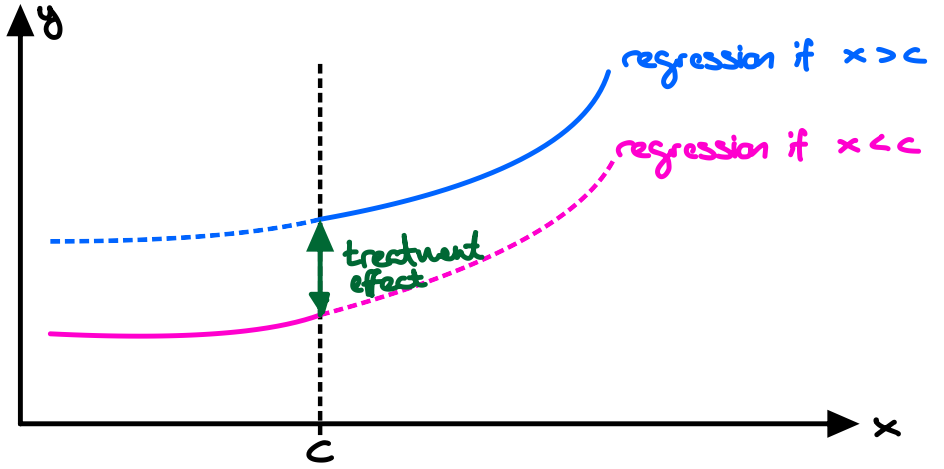
\includegraphics[width=.75\textwidth]{images/2017_18.png}
\end{figure}

Example: Let $x$ be time, $c$ is 1989, and $y$ the GDP growth in eastern Germany. Since the Berlin wall fell in 1989, it makes sense to model this as a regression discontinuity (ignoring the time series properties for the moment).
}
{
\subsubsection*{Exercise 4}

\begin{enumerate}[label=(\alph*)]
{\item 
$$
\begin{aligned}
f\left(x_{i}, b\right) & =y_{i}-\exp \left(x_{i} b\right) \\
f^{\prime}\left(x_{i}, b\right) & =-x_{i} \cdot \exp \left(x_{i} b\right) \\
\sqrt{n}(b-\beta) & \xrightarrow{d} N\left(0, \mathbb{E}\left(-x_{i} \exp \left(x_{i} \beta\right)\right)^{-2} \mathbb{E}\left(\exp \left(2 x_{i}\beta\right)\right)\right)
\end{aligned}
$$
}
{\item 

$$
\begin{aligned}
& \frac{\partial f\left(x_{i} b\right)}{\partial b}=\left[\begin{array}{l}
-\exp \left(x_{i} b\right) x_{i} \\
-\exp \left(x_{i} b\right) x_{i}^{2}
\end{array}\right] \\
& \sqrt{n}(b-\beta) \xrightarrow{d} N(0, \Sigma) \\
\Sigma&=A^{-1} B^{\prime} I_{2} S I_{2} B A^{-1} \\
A&=\mathbb{E}\left(\frac{\partial f(x_i b)}{\partial b}\right)^{\prime} I_{2} \mathbb{E}\left(\frac{\partial f(x_i b)}{\partial b}\right) \\
& =\mathbb{E}\left(\exp \left(x_{i} b\right) x_{i}\right)^{2}+\mathbb{E}\left(\exp \left(x_{i} b\right) x_{i}^{2}\right)^{2} \\
B&=\mathbb{E}\left(\frac{\partial f\left(x_{i} b\right)}{\partial b}\right)=\mathbb{E}\left[\begin{array}{l}
-\exp \left(x_{i} b\right) x_{i} \\
-\exp \left(x_{i} b\right) x_{i}^{2}
\end{array}\right] \\
S&=\operatorname{Var}\left(f\left(x_{i}, \beta\right)\right)=\operatorname{Var}\left[\begin{array}{c}
\varepsilon_{i} \\
\varepsilon_{i} x_{i}
\end{array}\right]=\mathbb{E}\left[\begin{array}{cc}
\varepsilon_{i}^{2} & x_{i} \varepsilon_{i}^{2} \\
x_{i} \varepsilon_{i}^{2} & x_{i}^{2} \varepsilon_{i}^{2}
\end{array}\right] \\
& =\mathbb{E}\left[\left.\mathbb{E}\left[\begin{array}{cc}
\varepsilon_{i}^{2} & x_{i} \varepsilon_{i}^{2} \\
x_{i} \varepsilon_{i}^{2} & x_{i}^{2} \varepsilon_{i}^{2}
\end{array}\right] \right\rvert\, x_{i}\right] \\
& =\mathbb{E}\left[\begin{array}{ll}
\exp (2 x_i \beta) & \exp (2 x_i \beta) x_{i} \\
\exp (2 x_i \beta) x_{i} & \exp (2 x_i \beta) x_{i}^{2}
\end{array}\right]
\end{aligned}
$$

\color{red}Done?\color{black}
}
\end{enumerate}
}
}
